\documentclass[a4paper,12pt]{article}
\usepackage{graphicx}
\usepackage{eso-pic}
\usepackage[utf8]{inputenc}
\usepackage[T1]{fontenc}
\usepackage[french]{babel}

\usepackage[colorlinks=True,citecolor=black,urlcolor=blue,linkcolor=black]{hyperref}
\usepackage{subfigure}
\usepackage[francais]{layout}
\usepackage{color}
\usepackage[table]{xcolor}
\usepackage{listings}
\usepackage{fancyhdr}
\lstset{
aboveskip=3mm,
belowskip=-2mm,
backgroundcolor=\color{darkWhite},
basicstyle=\footnotesize,
breakatwhitespace=false,
breaklines=true,
captionpos=b,
commentstyle=\color{red},
deletekeywords={...},
escapeinside={\%*}{*)},
extendedchars=true,
framexleftmargin=16pt,
framextopmargin=3pt,
framexbottommargin=6pt,
frame=tb,
keepspaces=true,
keywordstyle=\color{blue},
language=C,morekeywords={*,...},
numbers=left,
numbersep=10pt,
numberstyle=\tiny\color{black},
rulecolor=\color{black},
showspaces=false,
showstringspaces=false,
showtabs=false,
stepnumber=1,
stringstyle=\color{gray},
tabsize=4,
title=\lstname,
}


\usepackage[utf8]{inputenc}
\title{Projet jeu Darkest Dungeon}
\author{\textsc{Monjoux} Hugo & \textsc{Rivière} Hadrien & Option IS TP1}
\date{18 Septembre 2018}
\usepackage[a4paper,top=1.5cm,bottom=1.5cm,left=1.5cm,right=1.5cm,marginparwidth=1.75cm]{geometry}

\pagestyle{fancy}
\fancyhf{}
\chead{MONJOUX Hugo | RIVIERE Hadrien | Rendu 1.final | Page \thepage}

\begin{document}
\maketitle
\begin{figure}[!ht]
  \centering
  \includegraphics[width=1\textwidth]{Rendu1.1/ecran_acceuil.jpg}
  \caption{Aperçu du jeu "The Darkest Dungeon"}
\end{figure}

\newpage
\tableofcontents
\newpage
\section{Présentation Générale}
\subsection{Archétype}
Notre jeu s'inspire de Darkest Dungeon, qui est un RPG tour par tour, Rogue-like. Ce jeu est illustré dans les différentes figures exposées en fin du rapport. 

\subsection{Règles du jeu}

 Ce dernier permet au joueur d'évoluer soit en tant que héros, soit en tant qu'ennemis. L'objectif du joueur varie donc selon ce choix fait en début de partie. Si le joueur choisit de jouer en tant que héros, il doit arriver à la fin du niveau. Dans l'autre cas le joueur doit s'assurer que les héros n'arrive pas à la fin du niveau. 
\\ 
\indent
Le jeu se compose en trois vues : 
\begin{itemize}
    \item Vue d'accueil du joueur, qui pourra définir son équipe de héros, ainsi que l'inventaire de l'équipe, soit la répartition des ennemis sur les cartes de jeu
    \item Vue de déplacement dans le donjon
    \item Vue de combat lors de la confrontation des héros avec les ennemis
\end{itemize} 
\subsection{Ressources}
\begin{figure}[!ht]
  \centering
  \includegraphics[width=0.8\textwidth]{Rendu1.1/background3.jpg}
  \caption{Premier élément de décor : couloir}
\end{figure}
\begin{figure}[!ht]
  \centering
  \includegraphics[width=0.8\textwidth]{Rendu1.1/background4.jpg}
  \caption{Deuxième élément de décor : salle}
\end{figure}
\begin{figure}[!ht]
  \centering
  \includegraphics[width=1\textwidth]{Rendu1.1/ecran_acceuil.png}
  \caption{Ecran d'accueil avec à l'intérieur du cadre, le menu d'accueil (New game, Options...)}
\end{figure}
\begin{figure}[!ht]
  \centering
  \includegraphics[width=0.6\textwidth]{Rendu1.1/pers_licantrope.png}
  \caption{Exemple de design d'un personnage se transformant. Seulement les sprites encadrés seront utilisés pour alléger les ressources.}
\end{figure}
\begin{figure}[!ht]
  \centering
  \includegraphics[width=1\textwidth]{Rendu1.1/city1.png}
  \caption{Ville d'accueil du joueur avec de gauche à droite encadrés :  Auberge de recrutement pour modifier l'équipe, Sauvegarde de la progression, et Magasin pour remplir l'inventaire de l'équipe.}
\end{figure}
\begin{figure}[!ht]
  \centering
  \includegraphics[width=1\textwidth]{Rendu1.1/combat.png}
  \caption{Ecran de jeu principal : encadrés en gris clair, les héros à gauche et les ennemis à droite avec leur barre de vie respectives situées en dessous | encadrés en orange, les différents outils à dispositions du joueur (compétences, statistiques des personnages, équipements, carte, inventaire). Ces éléments seront adaptés aux contraintes de temps et de moyens de notre projet.}
\end{figure}
\clearpage
\newpage
\section{Description et conception des états}
\subsection{Description des états}
La partie, une fois le jeu lancée, est caractérisée par la paramétrisation du joueur et sa customisation de celle-ci lors de l'outgame. Notamment, le choix héros/ennemis évoqué ci-haut, la sauvegarde ou l'accès à un magasin pour remplir l'inventaire. 
\\ \indent
Puis une fois dans la partie ingame, l'état de jeu est formé par les éléments fixes (cartes, éléments de gameplay, ressources graphiques...) et des éléments mobiles (héros, ennemis, barres de vie, ordering lors des combats...). Les éléments mobiles dits vivants (héros et ennemis) sont répérés par une position sur une liste de salles existantes sur le donjon en cours d'exploration. 

\subsubsection{Etat éléments fixes}
Les différentes cartes, à l'instar de celles trouvables en FIGURE 6 et en bas à droite de la FIGURE 7, sont des cartes statiques présentant des ressources graphiques majoritairement statiques. L'ensemble de ces éléments ne seront intéractifs que par des effets de surbrillance ou d'ombre. 
\\ \indent
La \textbf{première carte illustrée en FIGURE 6} caractérisant la classe Village sert d'accueil au joueur souhaitant jouer côté Héros, et présentent un carrefour entre l'Auberge (constitution de l'équipe), l'Eglise (Sauvegarde), le Magasin (acheter des items pour l'inventaire de l'équipe), et le Carrosse (partir à la conquête des donjons). Sur cette carte on retrouve : 
\begin{itemize}
    \item Le Village : qui donne accès à la fois au Carrosse ainsi qu'à l'Eglise
    \item L'Auberge : qui donne accès à la customisation de l'équipe.
    \item Le Magasin : qui donne accès à un autre écran sur lequel le joueur peut acheter des items (Potions et autres items détaillés plus tard).
    \item Les Item : un listing des items obtenables par le Shop afin d'équiper le joueur au sein du Donjon, caractérisés par des méthodes singulières selon la nature de l'item.
\end{itemize}
\\ \indent
La \textbf{deuxième carte illustrée en FIGURE 7 en bas à droite} permet au joueur de se déplacer dans le donjon dans lequel il progresse. Cette carte intègre une unique ressource graphique qui est faite à la main, représentant le plan du donjon. Les salles, indiquées par des carrés, seront associées à des phéonomènes de surbrillance par exemple si le joueur s'y déplace.



\subsubsection{Etat élements mobiles}
Les éléments mobiles possèdent une position de départ qui correspond à leur position sur l'écran de combat avant que l'attaque soit effectuée. Ils ont ensuite une vitesse de déplacement qui correspond à la vitesse à la quelle le sprite se déplace sur l'écran. 

\begin{itemize}
\item Personnages (héros ou monstres): Ces éléments sont controllés soit par un humain soit par une IA. Leur mouvement correspondent aux choix faits par l'un d'entre eux. Les actions qui s'en suivent sont associées à ces choix mais sont prédéfinies dans le jeu (charge lors de l'attaque au corps à corps, personnage tremble après avoir reçu un coup, utilisation des skills...).
\item Icônes de personnages : ces icônes qui se situent en haut de l'écran de combat se déplacent en fonction du tour. Celle la plus à gauche correspond au personnage qui joue le plus tôt.
\end{itemize}
\newpage
\subsubsection{Etats généraux}
L'ensemble de ces états sont complétés par un état général qui résume l'état du jeu comme défini ci-dessous à un instant t : 
\begin{itemize}
    \item Une horloge permettant de rythmer les tours de jeu en ingame, ainsi que l'apparition et la désapparition des éléments in et outgame. 
    \item Le Gameplay du Game + est basé sur l'édition du nombre de donjons finis,
et du nombre de donjons finis successivement. Ainsi des conditionnelles sur ces chiffres peuvent être implémentées pour maximiser la durée de vie du jeu, ou simplement permettre de suivre le scoring du joueur sur sa partie. 
    \item L'Etat de l'équipe : la santé in-dungeon, l'état du personnage (en forme, en état de choc, empoisonné, mort...)
    \item L'état des salles du donjon visité : la liste des salles, leur occupation (nombre de monstres, quels monstres), leur état (finies, non finies, où le héros se situe).
    \item L'inventaire : il s'agit de lister l'ensemble des item qui à un moment t appartiennent au joueur. 
Il est à noter que la sauvegarde, comme évoqué plus haut en section 2.1.1, conserve les deux premiers tirets de ces états généraux. 
\end{itemize}

\subsection{Conception logicielle}
Le diagramme de classe est présenté ci-dessous en FIGURE 8 et nous pouvons y observer plusieurs groupes de classes: 
\begin{itemize}
    \item \textbf{Classes Elements :} ces classes sont représentées en jaune sur le diagramme pour les classes intermédiaires, les classes objets finales (qui n'ont pas de filles) sont représentées en bleue, et caractérisent des archétypes (d'item, de personnages ou d'ennemis). Afin d'identifier les natures des classes des méthodes sont définies telles que, notamment si l'objet créé est un élément mobile ou statique, par des méthodes isStatic(), ou au sein de l'architecture des classes statiques, pour savoir si l'objet créé est un bâtiment avec une méthode isBuilding(). 
    \item \textbf{Conteneurs d'élement :} en vert, les classes State, ElementTab, Inventaire et Team qui permettent d'accumuler les éléments utiles à la partie du joueur. Les trois classes Inventaire, Team et ElementTab sont des conteneurs d'objets qui sont à dimensions finies (des tableaux de dimensions N éléments), et la classe State qui nous permet d'accéder à toutes les données de l'état du jeu à un instant donné. 
\end{itemize}

\begin{figure}[!ht]
  \centering
  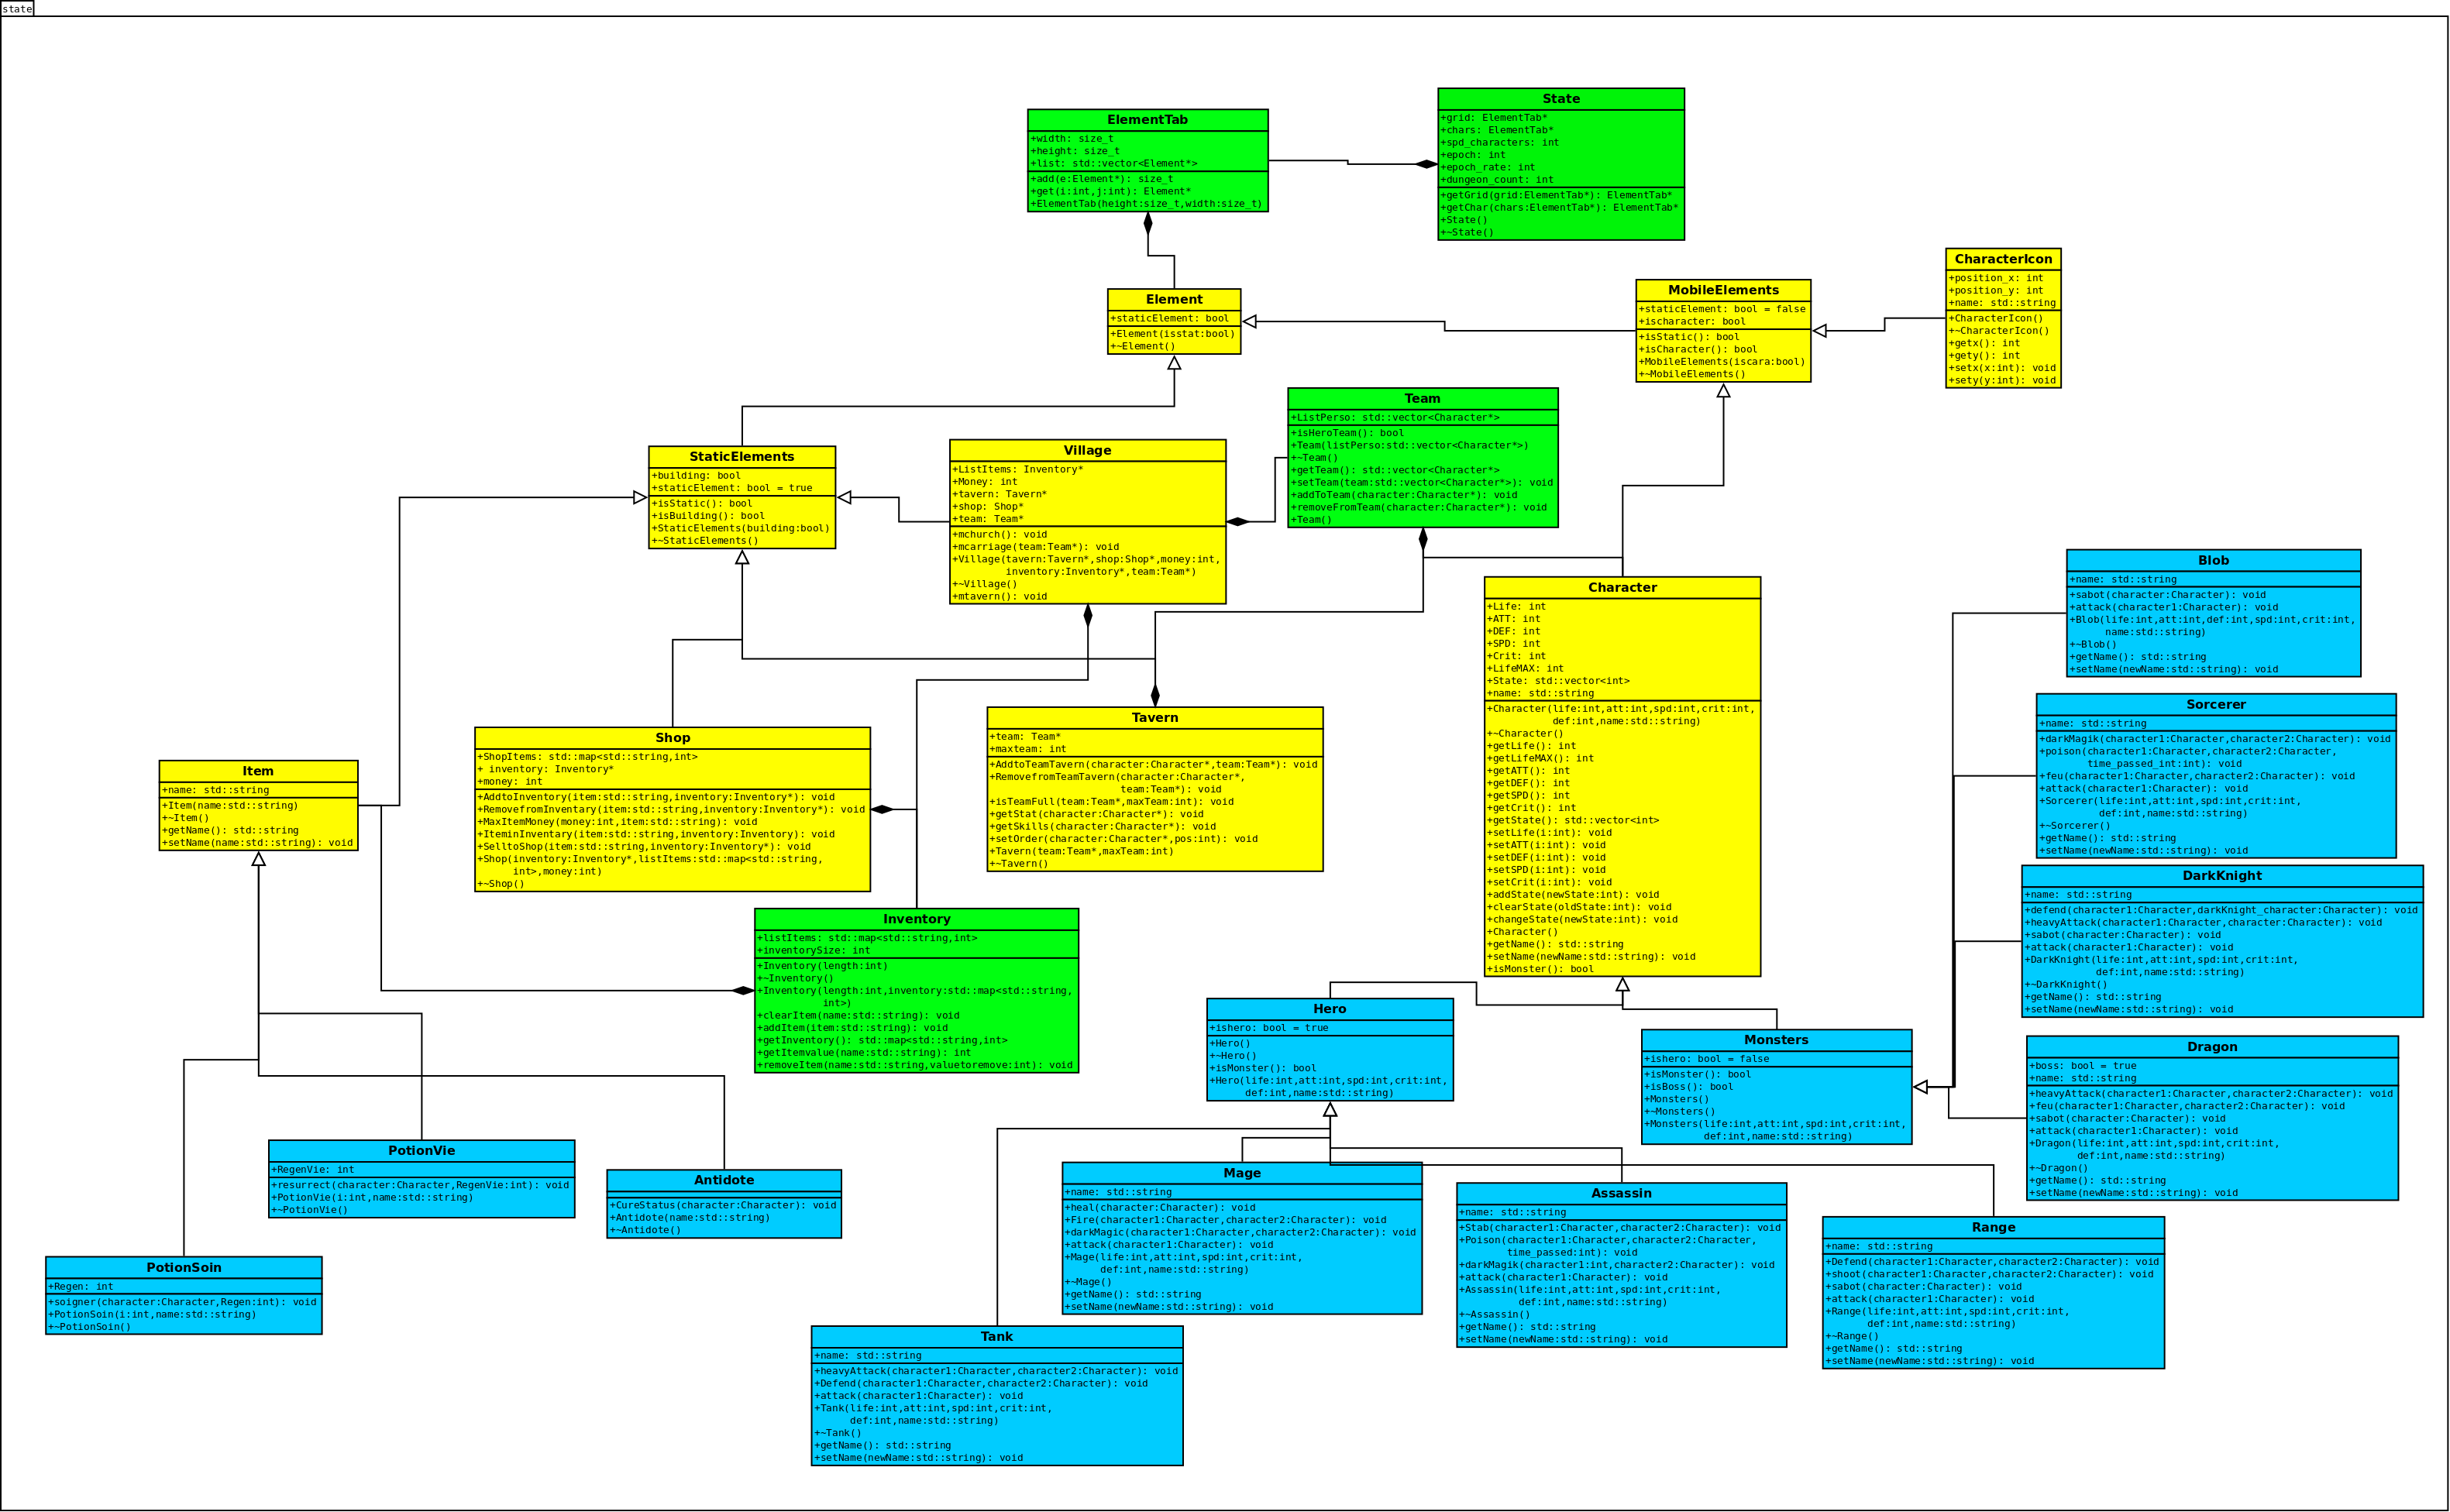
\includegraphics[angle=90,width=0.9\textwidth]{Rendu1final/state.png}
  \caption{Diagramme de classe associé au projet fait via DIA}
\end{figure}



\end{document}